\chapter{Results}
\label{sec:results}

In this section we show the performance of our two algorithms ($\thename$ and $\thenameoff$)
across a variety of continuous
control tasks.
First, we show $\thename$ performance in an off-policy setting on a toy example.
Then, we move to the fully off-policy setting, i.e. batch RL setting, and we test $\thenameoff$ performance
on several external datasets provided by the D4RL suite \citep{d4rl}.
In all the results we compare the policies learnt when maximizing for the expected value
(i.e. sampling $\tau \sim U([0,1])$,
from now on \textit{Mean})
and when maximizing for the $\alpha$-CVaR (i.e. sampling $\tau \sim U([0,\alpha])$,
from now on \textit{CVaR}).

\section{Off-policy setting}
We test the performance of $\thename$ algorithm in an off-policy setting.
We show that when the reward is deterministic the policies learnt by \textit{Mean} and \textit{CVaR} are the same.
When adding uncertainty, we show how the policies differ to maximize their respective objective functions.
\subsection{Car to goal}

A car with fully-observable 2D-state: [position, velocity] must move to a goal
position $x_F=\SI{2.5}{\metre}$ starting at rest $(x_0=\SI{0.0}{\metre}, v_0=\SI{0.0}{\metre\per\s}$).
The car can control its acceleration $a$ which is constrained to range between 
[-1.0,1.0]\si{\metre\per\square\s} every $\Delta k=0.1$ seconds.
Per every time step $k$ before reaching the goal the car receives a penalization
$R_{k}=-10$.
If the car reaches the goal position, it receives a reward $R_F=+370$ and the episode ends.
Otherwise, after $T_F=400k$ the episode ends (with no extra penalization).
We model the dynamics using a simple rectilinear uniform acceleration motion that updates
the states of the agent at at every time step $k$:
\begin{align}
        v_{k+1} = v_k + a\Delta{k}\\
        x_{k+1} = x_{k} + v_{k} \Delta{k} + 0.5a_{k} \big (\Delta k \big )^2      
\end{align}

In the following, we test performance of the algorithm in 3 different settings.
The first 2 settings, with no uncertainty, are meant to show that the algorithm is able to learn
meaningful policies depending on the reward function used.
The first setting has no extra modifications in the rewards and shows that for both
\textit{Mean} and \textit{CVaR} the car learns to reach the goal 
in the shortest time possible.
The second setting adds an extra penalization when velocity exceeds a certain value  with probability 1.
Since there is no uncertainty, in both
\textit{Mean} and \textit{CVaR} the car learns to accelerate till
the threshold velocity is reached and keeps without exceeding maximum velocity till the goal.\\
In the third setting we show how the 2 policies differ when
penalization for high velocity occurs with low probability.
\textit{Mean} ignores the low probability penalizations and 
learns same policy as for setting 1, whereas \textit{CVaR} evolves to a 
risk-sensitive policy and learns same policy as in setting 2
to ensure high penalizations do not occur.
\subsection{Setting 1: No velocity penalization}
Car arrives at the goal position with maximum acceleration throughout the whole episode
for both \textit{Mean} and \textit{CVaR}.
Car keeps an acceleration of $\SI{1}{\metre\per\square\ts}$ for the whole episode and hence reaches $x_F=2.5$\si{\metre} in 24 time steps.
Hence the final cumulative reward $G_T= (24-1) R_{k} + R_{F}=140$.

\begin{figure}[ht]
        \centering
        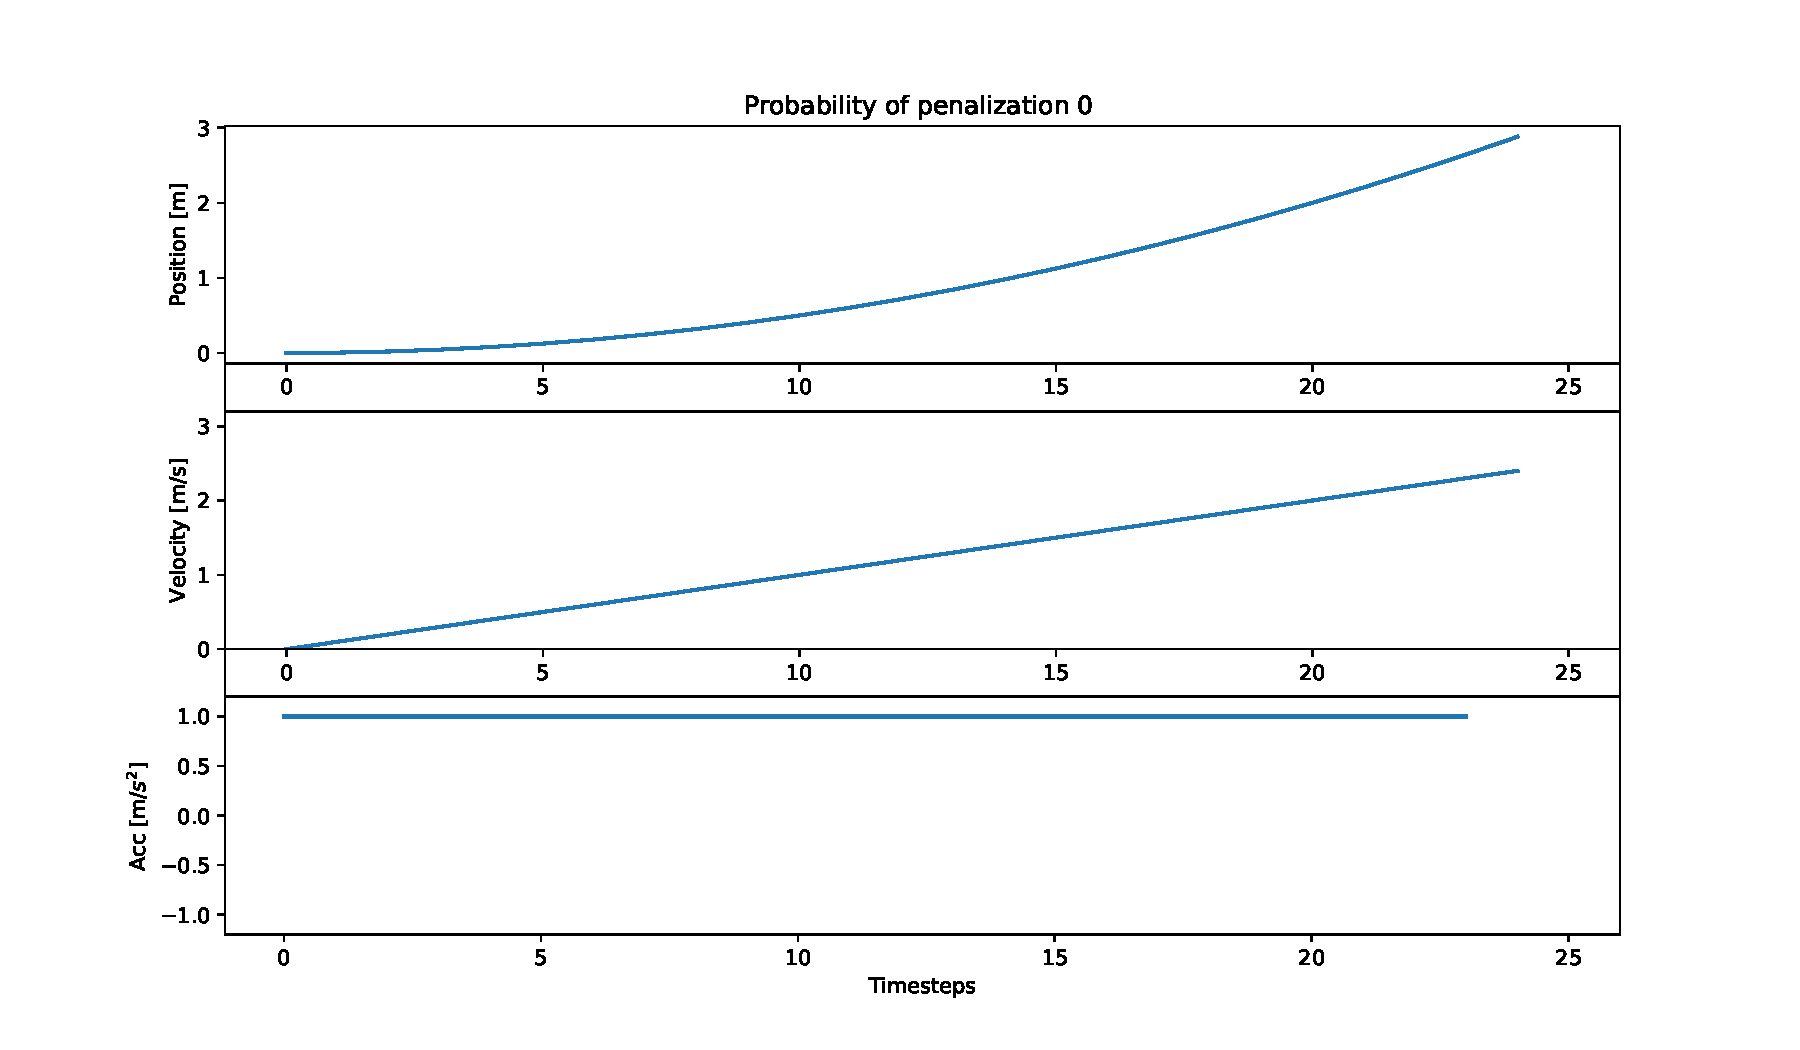
\includegraphics[width=0.8\textwidth]{images/Car/CVAR/Trajectory_nopenal.pdf}
        \caption{States and control evolution during evaluation without velocity penalization. 
         Learnt policy is the same for both \textit{Mean} and \textit{CVaR}}
        \label{fig:traj1_nopenal}
    
\end{figure}

\subsection{Setting 2: Velocity penalization with probability 1 }
When the car velocity exceeds 1\si{\metre\per\ts} it receives a penalization of $R_v=-25$.
We expect both \textit{CVaR} and \textit{Mean} to learn similar policies 
since there is no reward uncertainty. As expected
both learn to accelerate with maximum value
until a velocity of 1\si{\metre\per\ts} is reached
and then they keep with 1\si{\metre\per\ts} velocity until the goal.

Starting from $x_0=0$\si\metre, the car reaches a velocity of 1\si{\metre\per\ts} after 
10 time steps, at $x_{k=10}=0.5$. Keeping velocity 1\si{\metre\per\ts} through 
the rest of the episode, it reaches the goal position after $21$ time steps, i.e. in a total of 31 steps.
Hence the final cumulative reward $G_T= (31-1) R_{k} + R_{F}=70$.

We notice that the reward values were deliberately chosen in order to ensure that for the Setting 2,
driving faster than 1\si{\metre\per\ts} never induces higher cumulative
rewards. In that hypothetic case, car will reach goal in 24 time steps
but would add penalization for driving over the speed limit for 10 time steps:\\
$G_T= (24-1)R_{k} + (21-1)R_{v} + R_{F} << (31-1) R_{k} + R_{F}=70$

\begin{figure}[ht]
        \centering
        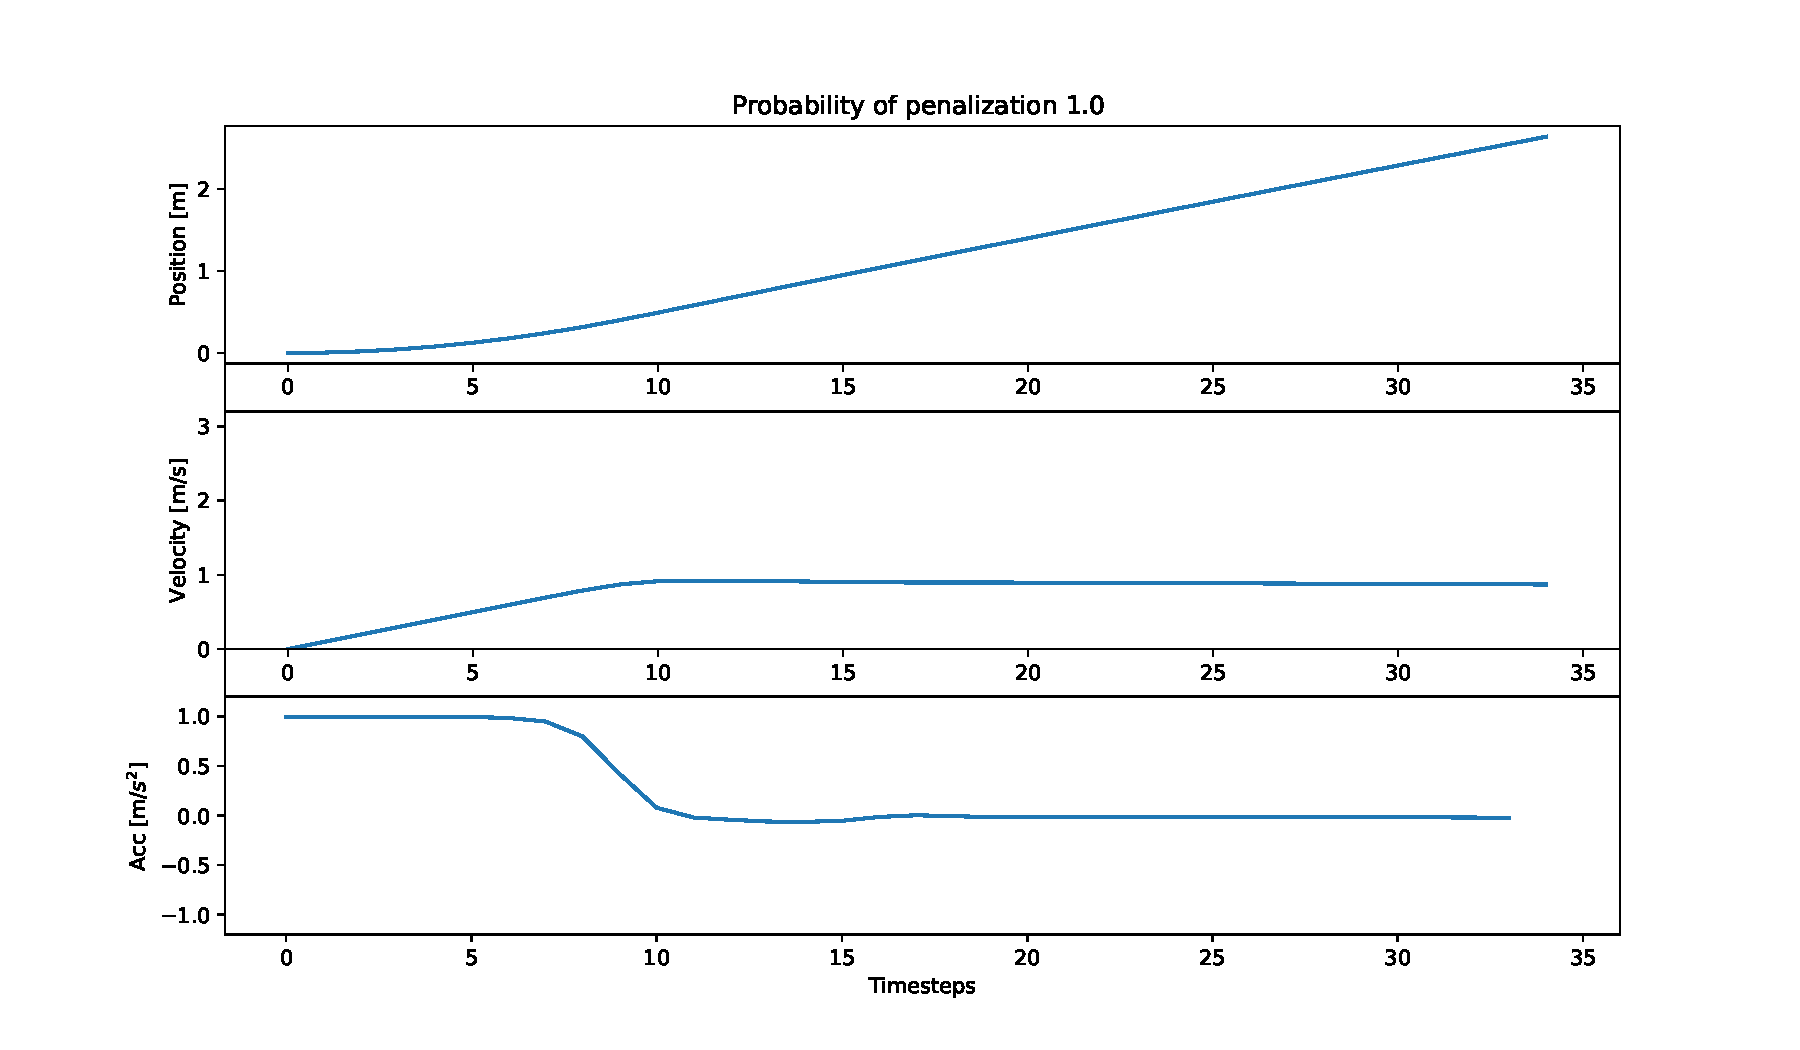
\includegraphics[width=0.8\textwidth]{images/Car/CVAR/Trajectory_penal.pdf}
        \caption{States and control evolution during evaluation with velocity penalization
        with probability 1.
        Learnt policy is the same for both \textit{Mean} and \textit{CVaR}}
        \label{fig:traj1_penal1}
    
\end{figure}

\newpage
\subsection{Case 3: Velocity penalization with probability P=0.2 }
When penalization only occurs with a certain low probability P=0.2, we can notice a difference
in the policies learnt by \textit{CVaR} and \textit{Mean}.
\textit{Mean} learns policies so that it maximizes the expected
value by keeping a linear increase of the velocity during the whole episode disregarding the low probability events with high penalizations,
whereas \textit{CVaR} saturates the velocity, even though the
probability of a penalization is low.

In the following we show the evaluation during training for both \textit{Mean} and
\textit{CVaR}.
Specifically, every 5 training episodes, we test the current policy over 500 evaluation episodes.
During evaluation, we remove the exploration noise from the policy.
During this 500 evaluation episodes, we compute the mean of the cumulative rewards (see Figure \ref{fig:mean_car}),
the CVaR with a confidence level of 0.1  (see Figure \ref{fig:cvar_car}) and also the mean of the number of times the 
maximum velocity is exceeded  (see Figure \ref{fig:maxveltimes_car}). 

After training, we used the final policies and deployed them in the 
environment. Obtained trajectories are shown in Figure \ref{fig:traj_probpenal0.2}.
A histogram of the resulting cumulative rewards shows
how the \textit{Mean} algorithm obtains, in average, higher cumulative rewards, but in some scenarios it 
obtains really low results, whereas the \textit{CVaR} performs in average worse than \textit{Mean} 
but the conditional value-at-risk is higher than for the \textit{Mean} (see Figure \ref{fig:histogram_cvar_vs_mean})

\begin{figure}[ht]
        \centering
        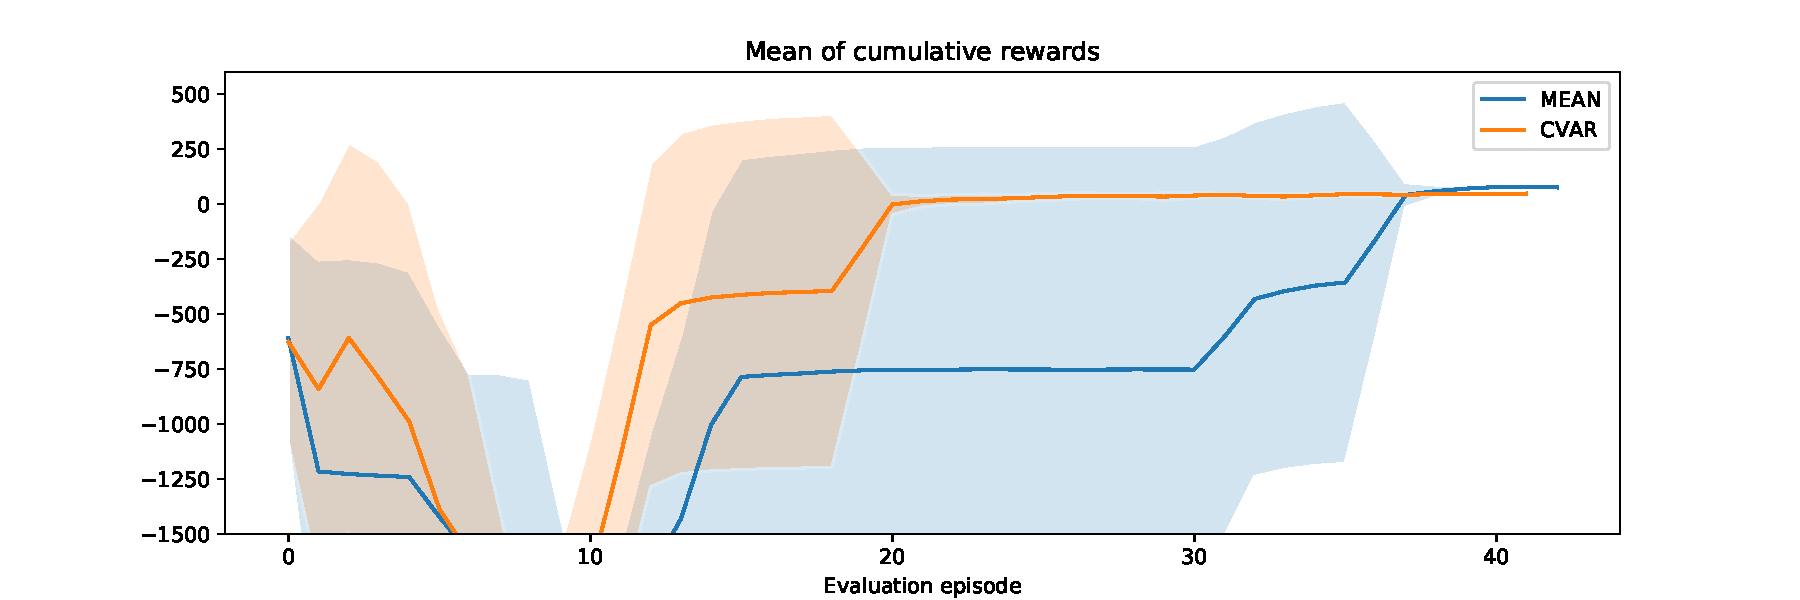
\includegraphics[width=0.8\textwidth]{images/Car/CVAR/mean_train_withstds.pdf}
        \caption{Evolution of mean of the cumulative rewards over 500 evaluation episodes.
        Every datapoint corresponds
        to one evaluation process performed every 10 training episodes.For the plot we
        show averaged values over 5 random seeds and 1 std}
        \label{fig:mean_car}
    
\end{figure}

\begin{figure}[ht]
        \centering
        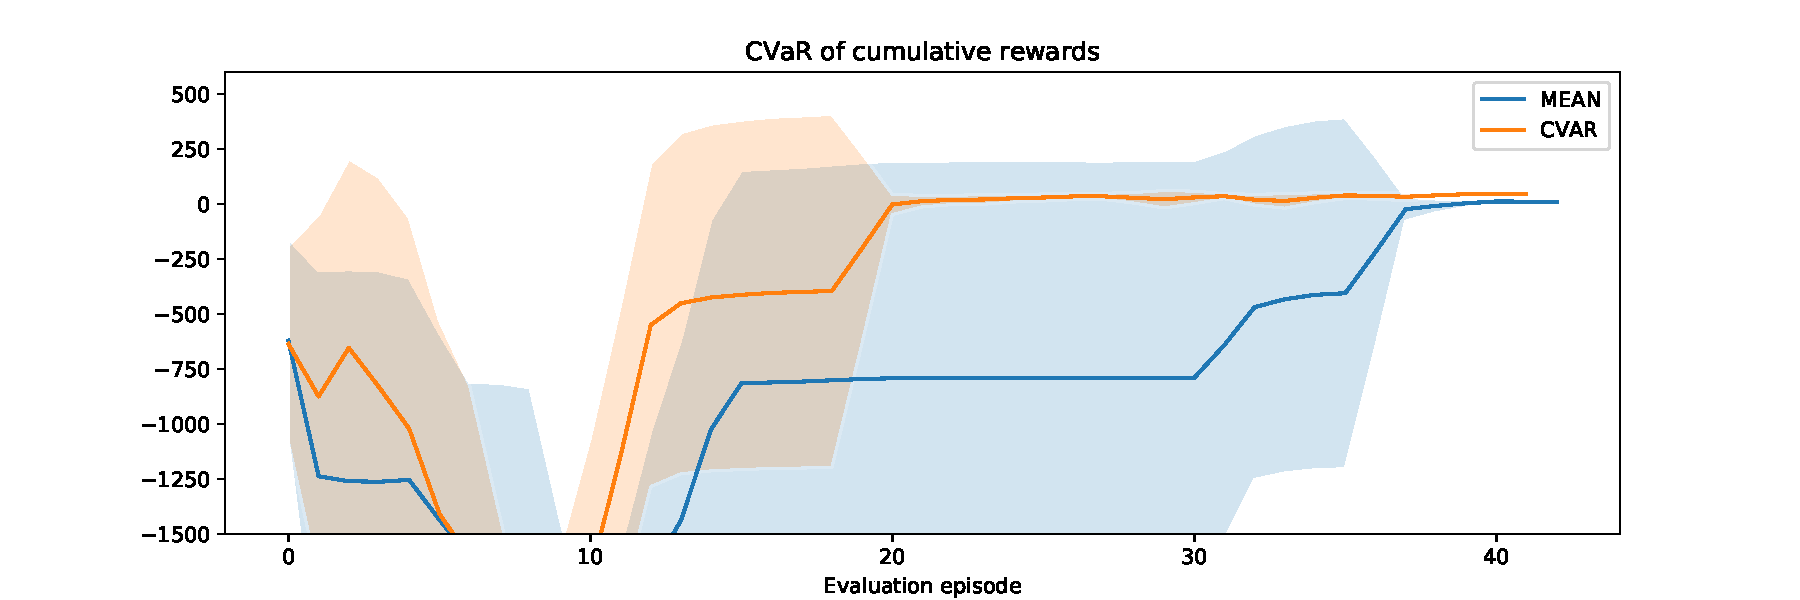
\includegraphics[width=0.8\textwidth]{images/Car/CVAR/cvar_train_withstds.pdf}
        \caption{Evolution of CVaR$_\alpha=0.1$ of the cumulative rewards over 500 evaluation episodes.
        Every datapoint corresponds
        to one evaluation process performed every 10 training episodes.
        For the plot we
        show averaged values over 5 random seeds and 1 std}
        \label{fig:cvar_car}
    
\end{figure}

\begin{figure}[ht]
        \centering
        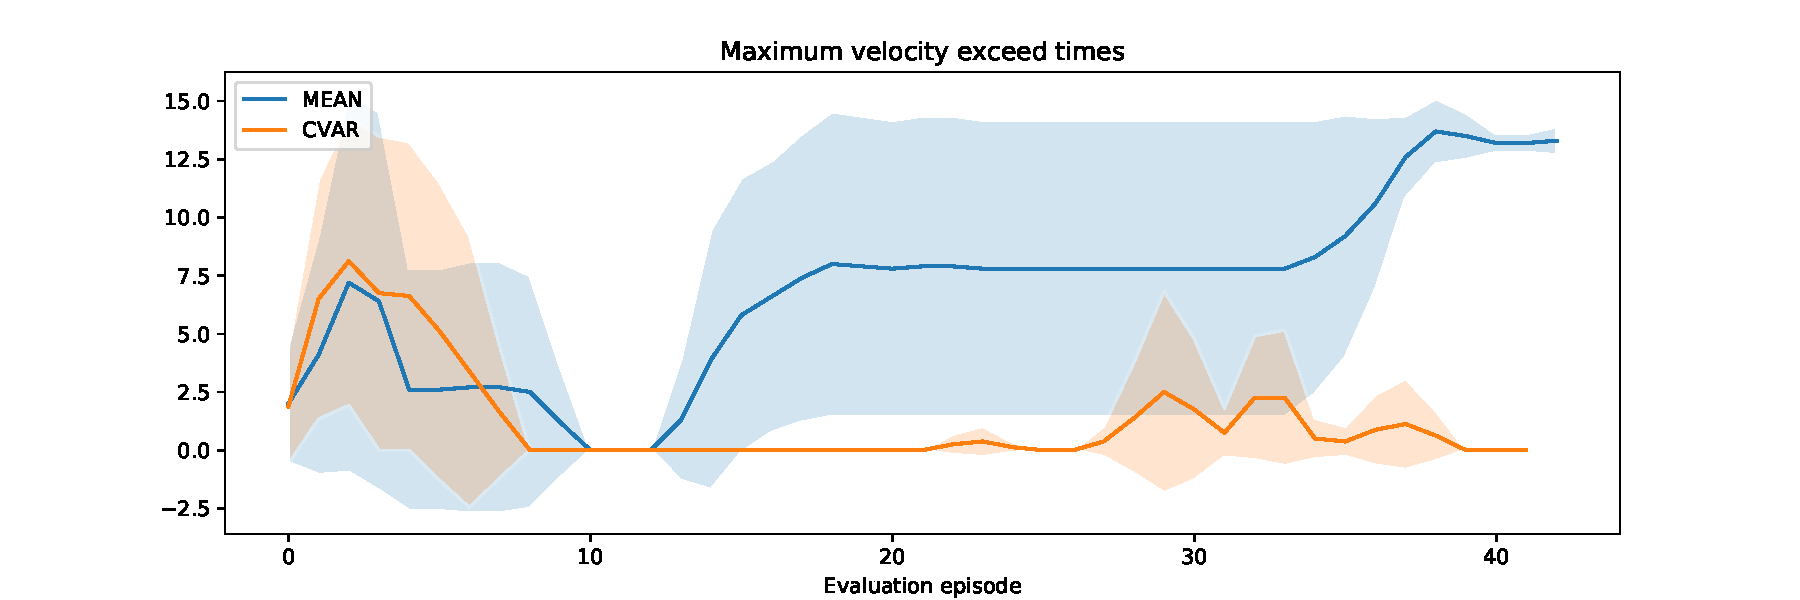
\includegraphics[width=0.8\textwidth]{images/Car/CVAR/times_exceedvel_withstds.pdf}
        \caption{Evolution of number of times penalized velocity is exceeded.
        Every datapoint corresponds
        to one evaluation process performed every 10 training episodes. For the plot we
        show averaged values over 5 random seeds and 1 std}
        \label{fig:maxveltimes_car}
    
\end{figure}

\begin{figure}[ht]
        \centering
        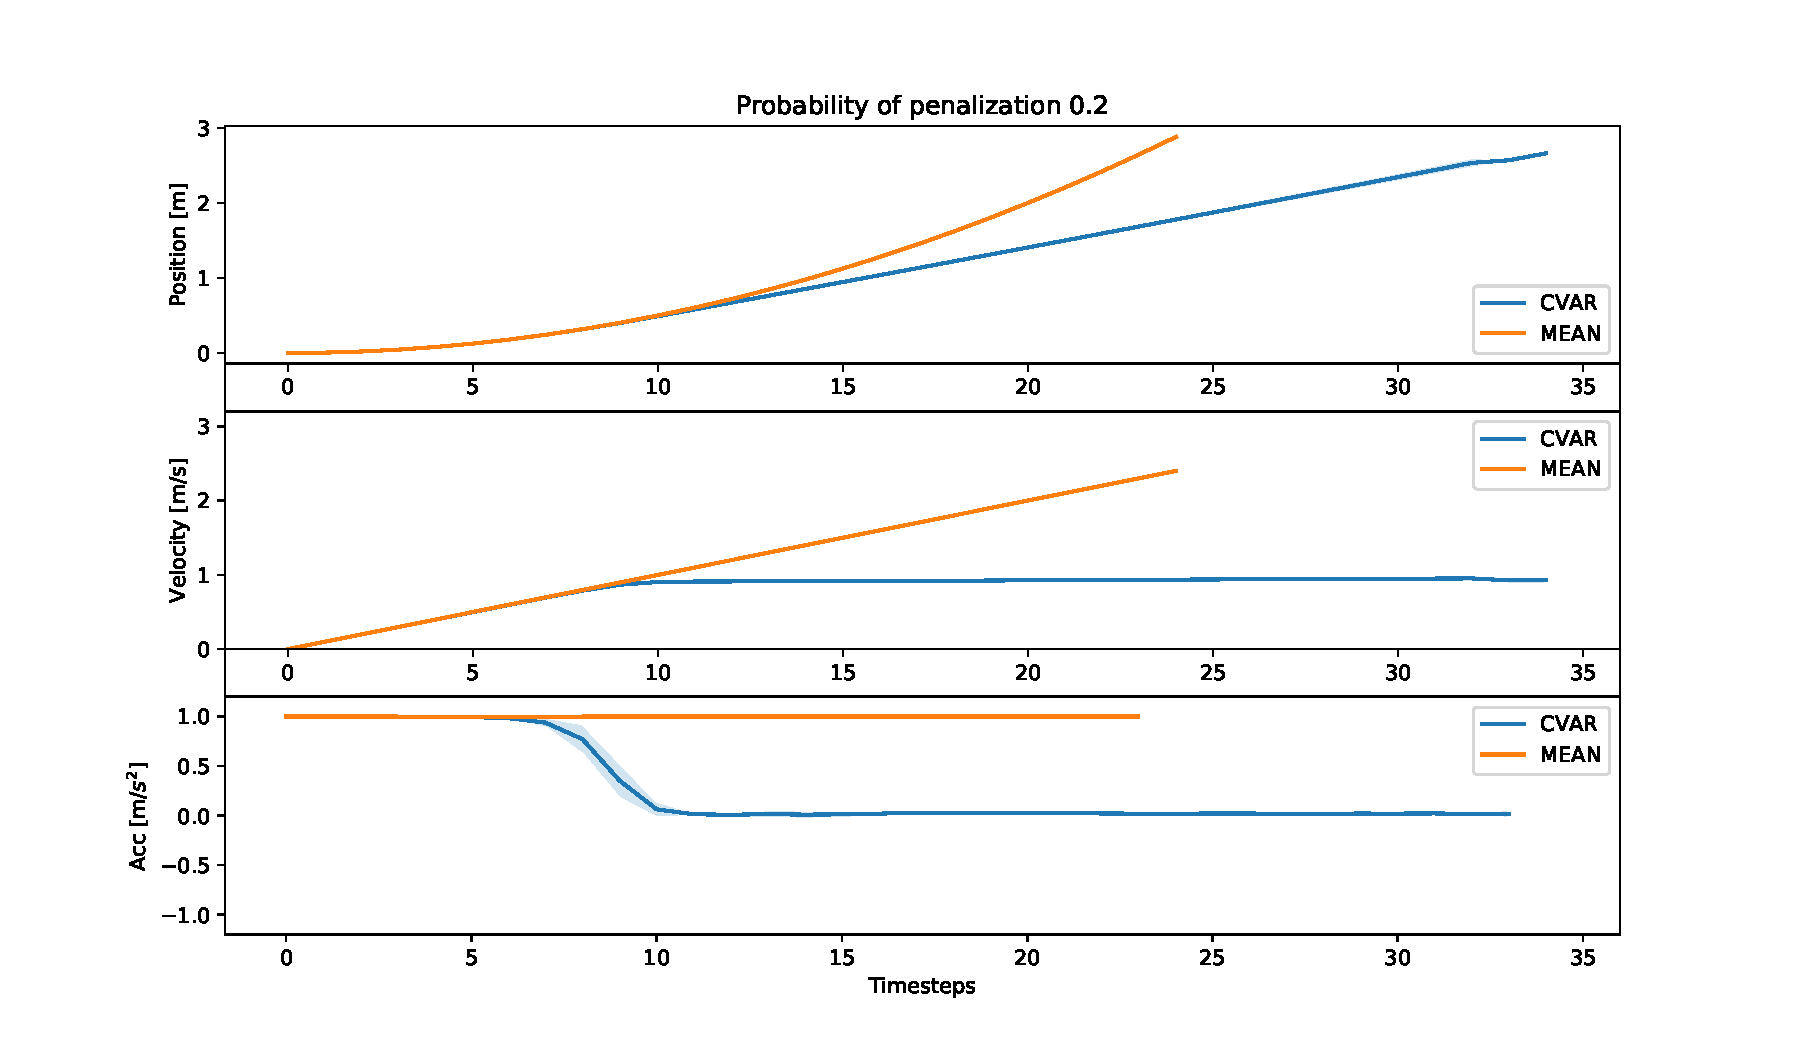
\includegraphics[width=0.8\textwidth]{images/Car/CVAR/Trajectory_withstds_penal.pdf}
        \caption{States and control evolution during evaluation with velocity penalization
        with probability 0.2.
        Learnt policies by \textit{Mean} and \textit{CVaR} differ, \textit{CVaR} leading
        towards risk-averse behavior}
        \label{fig:traj_probpenal0.2}
    
\end{figure}


\begin{figure}[ht]
        \centering
        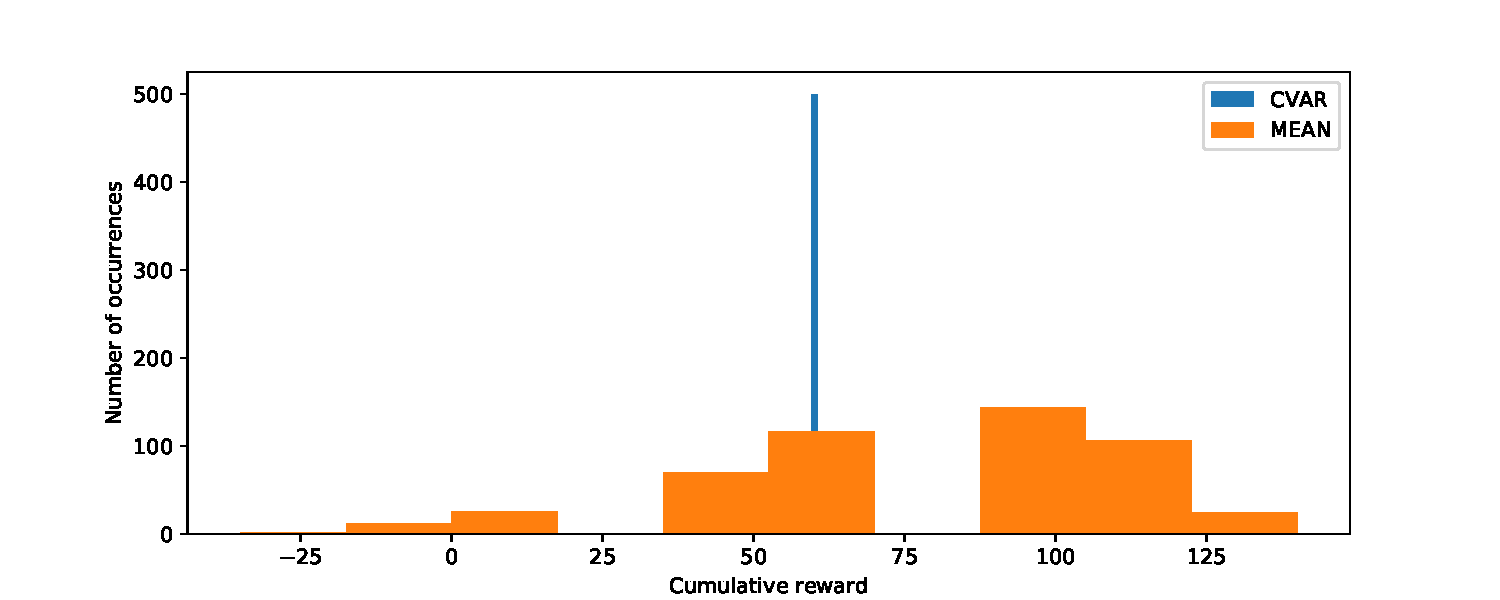
\includegraphics[width=0.8\textwidth]{images/Car/histogram_rewards1vs01.pdf}
        \caption{Comparison of cumulative rewards achieved with \textit{CVaR} and \textit{Mean}
        when the probability of velocity penalization is 0.2.
        \textit{Mean} achieves a higher expected value  ($\mu=78.1)$  but 
        has a lower CVAR ($\text{CVaR}_{\alpha= 0.1}$=12) compared to
        \textit{CVaR} ($\mu=60$ and $\text{CVaR}_{\alpha= 0.1}$=60).
        Data was obtained by acting for 500 episodes with the trained policies.
        Distribution of rewards for \textit{Mean} follows a binomial distribution B(n,p)
        with n being the number of steps with a velocity higher than the penalized and 
        p the probability of penalization.}
        \label{fig:histogram_cvar_vs_mean}
    
\end{figure}


